%%%%%%%%%%%%%%%%%%%%%%%%%%%%%%%%%%%%%%%%%
% Stylish Article
% LaTeX Template
% Version 2.2 (2020-10-22)
%
% This template has been downloaded from:
% http://www.LaTeXTemplates.com
%
% Original author:
% Mathias Legrand (legrand.mathias@gmail.com) 
% With extensive modifications by:
% Vel (vel@latextemplates.com)
%
% License:
% CC BY-NC-SA 3.0 (http://creativecommons.org/licenses/by-nc-sa/3.0/)
%
%%%%%%%%%%%%%%%%%%%%%%%%%%%%%%%%%%%%%%%%%

%----------------------------------------------------------------------------------------
%	PACKAGES AND OTHER DOCUMENT CONFIGURATIONS
%----------------------------------------------------------------------------------------

\documentclass[fleqn,10pt]{SelfArx} % Document font size and equations flushed left

\usepackage[english]{babel} % Specify a different language here - english by default
\usepackage[numbers]{natbib}
\usepackage{url}
\usepackage{lipsum} % Required to insert dummy text. To be removed otherwise

\usepackage{tcolorbox}
\usepackage{siunitx}
\tcbuselibrary{xparse}
\sisetup{
    group-digits=true,
    group-separator={\,},
}
%----------------------------------------------------------------------------------------
%	COLUMNS
%----------------------------------------------------------------------------------------

\setlength{\columnsep}{0.55cm} % Distance between the two columns of text
\setlength{\fboxrule}{0.75pt} % Width of the border around the abstract

%----------------------------------------------------------------------------------------
%	COLORS
%----------------------------------------------------------------------------------------

\definecolor{color1}{RGB}{0,0,90} % Color of the article title and sections
\definecolor{color2}{RGB}{0,20,20} % Color of the boxes behind the abstract and headings

%----------------------------------------------------------------------------------------
%	HYPERLINKS
%----------------------------------------------------------------------------------------

\usepackage{hyperref} % Required for hyperlinks

\hypersetup{
	hidelinks,
	colorlinks,
	breaklinks=true,
	urlcolor=color2,
	citecolor=color1,
	linkcolor=color1,
	bookmarksopen=false,
	pdftitle={Title},
	pdfauthor={Author},
}

%----------------------------------------------------------------------------------------
%	ARTICLE INFORMATION
%----------------------------------------------------------------------------------------

\JournalInfo{Data Scientist Nanodegree} % Journal information
\Archive{Capstone Project} % Additional notes (e.g. copyright, DOI, review/research article)

\PaperTitle{Short Term Stock Price Prediction with Machine Learning} % Article title

\Authors{Lucas Breinlinger\textsuperscript{1}} % Authors
\affiliation{\textsuperscript{1}\textit{Contact: lucasbr@me.com}} % Author affiliation


\Keywords{} % Keywords - if you don't want any simply remove all the text between the curly brackets
\newcommand{\keywordname}{Keywords} % Defines the keywords heading name

%----------------------------------------------------------------------------------------
%	ABSTRACT
%----------------------------------------------------------------------------------------

\Abstract{Accurately predicting stock prices is a highly sought after mastery. In recent developments Long Short Term Memory, a type of recurrent neural network, have proven to be highly promising in achieving better predictions.
todo: add 3-10 sentences blabla + result + methodology}

%----------------------------------------------------------------------------------------

\begin{document}

\maketitle % Output the title and abstract box

\tableofcontents % Output the contents section

\thispagestyle{empty} % Removes page numbering from the first page

%----------------------------------------------------------------------------------------
%	ARTICLE CONTENTS
%----------------------------------------------------------------------------------------

\section{Project Definition} % The \section*{} command stops section numbering

The accurate forecast of stock prices, traded on an exchange, is inarguably one of the most challeging topics in the field of asset pricing. The stock market is described as a unpredictable, dynamic and non-linear construct. Predicting the prices of its stocks is a ambitious undertaking and depends on many variables including but not limited to global economy, company's metrics and local and global political situation. 

Historically there are two main prediction metods. The fundamental analysis which is a qualitative analysis of the company is interested in finding the true value of a stock and compare it to the actual traded value. The evaluator utilizes several performance criterias e.g. the P/E ratio in order to truely assess the underlying stock. Secondly, the technical analysis, which is solely based on the past price of the stock e.g. in form of closing or opening prices as time-series. Its rather a short term predicing using factors like the Moving Average (MA) or the Exponential Moving Average (EMA). Its basic assumption is that every significant information about the stock is already considered in the stock price.

The fast computational development has led to the point that Machine learning techniques have a significant application in financial problem. The use of artificial neural networks have found more and its way into the field of stock price prediction. Here a recurrent neural network (RNN) has found very proven, more precisely the Long Short Term Memory (LSTM). Its advantage being
able to process entire sequences of data rather than only one single data point. It has proven to be very practial with time series data such our historical stock prices. 

In this project, I create an application which is going to predict the \textbf{closing price} of any given stock for which it is trained on. For the sake of convenience this report only considers the stock price prediction of the \textbf{Apple} Inc. (\textit{\$AAPL}) stock.

A train-test cycle is used to test the accuracy of the prediction. The root mean squared error (\ref{eq.rmse}) is used to measure the accuracy of the mode:
\begin{equation}
RMSE = \sqrt{\dfrac{\Sigma_{i}(\hat{y}_i-y_i)}{N}} 
\label{eq.rmse}
\end{equation}
where $\hat{y}_i$ is the prediction of the $i-th$ stock price $y_i$ and $N$ is the total number of predicted stock prices.


%------------------------------------------------

\section{Data Analysis}

\begin{table*}[hbt]
	\caption{First lines of \textit{Apple Inc.} stock prices dataset}
	\centering
\begin{tabular}{lllrrrr S[table-auto-round,table-format=9.0] rr}
\toprule
Ticker &       Name &       Date &  Open &  High &   Low &  Close &       {Volume} &  Dividends &  Stock Splits \\
\midrule
  AAPL & Apple Inc. & 2012-07-19 & 18.77 & 18.90 & 18.61 &  18.87 & 436861600.00 &       0 &          0 \\
  AAPL & Apple Inc. & 2012-07-20 & 18.83 & 18.87 & 18.54 &  18.56 & 397471200.00 &       0 &          0 \\
  AAPL & Apple Inc. & 2012-07-23 & 18.25 & 18.61 & 18.05 &  18.54 & 487975600.00 &       0 &          0 \\
  AAPL & Apple Inc. & 2012-07-24 & 18.65 & 18.72 & 18.38 &  18.45 & 565132400.00 &       0 &          0 \\
  AAPL & Apple Inc. & 2012-07-25 & 17.64 & 17.84 & 17.51 &  17.66 & 877312800.00 &       0 &          0 \\
\bottomrule
\end{tabular}
	\label{tab:df.head}
\end{table*}

\begin{table*}[hbt]
	\caption{Statistics of the Apple stock prices. Which represent our used features}
	\centering
\begin{tabular}{lS[table-auto-round,table-format=9.1] S[table-auto-round,table-format=9.1] S[table-auto-round,table-format=9.1] S[table-auto-round,table-format=9.1]S[table-auto-round,scientific-notation = engineering, table-format=-1.1e-1]  S[table-auto-round,table-format=9.0]}
\toprule
{} &         {Open} &         {High} &          {Low}&        {Close}              \\
\midrule
count &  2514.000000 &  2514.000000 &  2514.000000 &  2514.000000  \\
mean  &    54.976304 &    55.586809 &    54.385991 &    55.010195 \\
std   &    45.998891 &    46.593796 &    45.425948 &    46.036470  \\
min   &    12.090742 &    12.453181 &    12.001301 &    12.170523  \\
25\%   &    22.846671 &    23.103172 &    22.672594 &    22.848148 \\
50\%   &    36.503730 &    36.712400 &    36.239020 &    36.499804  \\
75\%   &    66.667990 &    68.501637 &    65.989975 &    67.521479  \\
max   &   182.630005 &   182.940002 &   179.119995 &   182.009995  \\
\bottomrule
\end{tabular}
	\label{tab:df.statistrics}
\end{table*}


The dataset was collected with the help of \tcboxverb{yfinance} python plugin. In my case it is replacing the not working Yahoo Finance API. The collected dataframe contains
\begin{itemize}[noitemsep] % [noitemsep] removes whitespace between the items for a compact look
	\item \num{1108837} rows
	\item $10$ columns
	\item price information for $457$ unique stocks
	\item Data of the last 10 years (including 17/07/2022)
\end{itemize} and was collected on the 18/07/2022. I use a list of 457 randomly selected stock tickers to generate the dataset. 

The structure and the first 5 lines of the table filtered for \textit{Apple Inc.} are displayed in table \ref{tab:df.head}. For each day and each stock (denoted by its ticker (\textit{Ticker}) and company name (\textit{Name}) the dataset contains the price of the stock in dollar 
when opening the market (\textit{Open}), closing the market (\textit{Close}). Furthermore there the days lowest (\textit{Low}) and highest 
intra-day price (\textit{High} is available, as well as the daily traded volume (\textit{Volume}).


Looking at the \textit{Apple Inc.} stock there are 2514 columns regarding the apple stock with a minimum closing price of $12.17$ and a maximum closing price of $182.01$. There are no missing values (see table \ref{tab:df.statistrics}) in the dataset, and the date and value columns are correctly set as a datetime respectively float columns. In table \ref{tab:df.statistrics} the statistics of the distinctive variables are shown.

\begin{figure}[ht]\centering
	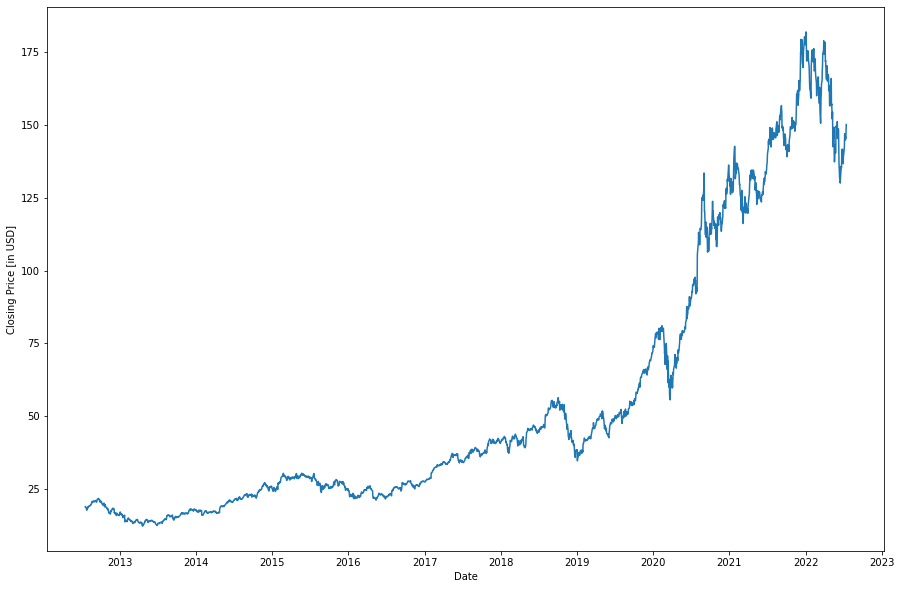
\includegraphics[width=\linewidth]{closing}
	\caption{Closing price of the \textit{Apple Inc.} in the last 10 years.}
	\label{fig:results}
\end{figure}

In figure \ref{fig:results} the highly volatile closing price of the stock is shown for its last 10 years. In recent years the stocke prices have incresead roughly sevenfold. 




%------------------------------------------------

\section{Methodology}

\begin{figure*}[ht]\centering % Using \begin{figure*} makes the figure take up the entire width of the page
	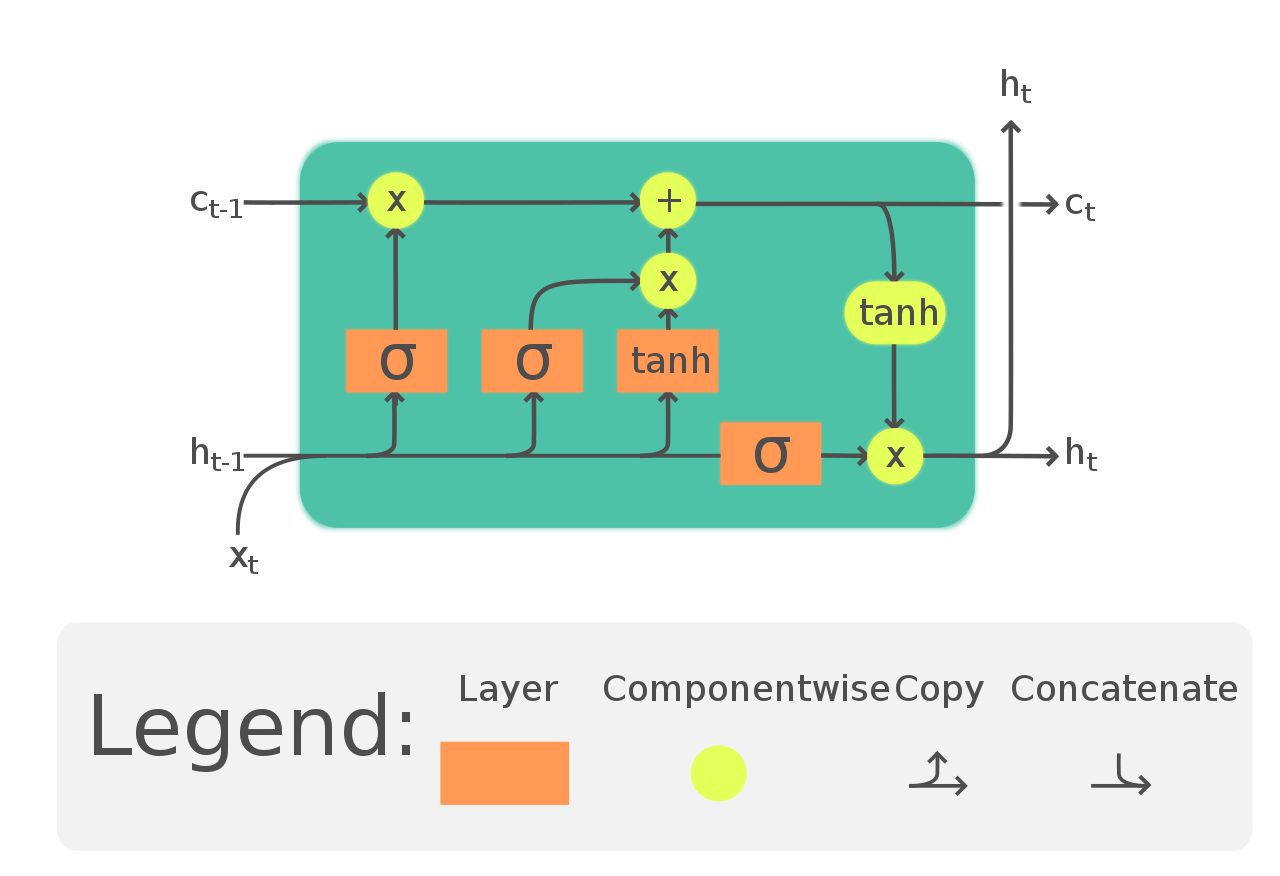
\includegraphics[width=\linewidth]{LSTM}
	\caption{The reccurent cell of a LSTM network \cite{LSTM}.}
	\label{fig:lstm.network}
\end{figure*}
In figure \ref{fig:lstm.network} a recurrent cell of a LSTM network is shown.

In order for the neural network to work properly the stock prices have to be normalized. This will help our model to converge faster and be more stable. Furthermore when using the scaler on the input features with different scales all features will contribute equally to the fitting and there will be no bias due to a different scaling. I am using the MinMaxScaler (\ref{eq.minmax}) of sci-kit learn.
\begin{equation}
x_{i,scaled}=\dfrac{x_i-min(x)}{max(x)-min(x)}
\label{eq.minmax}
\end{equation}



\subsection{Data Preprocessing}

\lipsum[11] % Dummy text



\subsubsection{Subsubsection}

\lipsum[12] % Dummy text

\begin{description}
	\item[Word] Definition
	\item[Concept] Explanation
	\item[Idea] Text
\end{description}

\subsubsection{Subsubsection}

\lipsum[13] % Dummy text

\begin{itemize}[noitemsep] % [noitemsep] removes whitespace between the items for a compact look
	\item First item in a list
	\item Second item in a list
	\item Third item in a list
\end{itemize}

\subsubsection{Subsubsection}

\lipsum[14] % Dummy text

\subsection{Implementation}

\lipsum[15-23] % Dummy text

\subsection{Refinement}

\lipsum[15-23] % Dummy text

\section{Results}
\lipsum[15-23] % Dummy text
\section{Conclusion}
\lipsum[15-23] % Dummy text


%------------------------------------------------



%----------------------------------------------------------------------------------------
%	REFERENCE LIST
%----------------------------------------------------------------------------------------

\phantomsection
\addcontentsline{toc}{section}{References} % Adds this section to the table of contents
\bibliographystyle{unsrt}
\bibliography{sample.bib}

%----------------------------------------------------------------------------------------

\end{document}